\documentclass[a4paper,english,12pt]{article}
\usepackage{%
	amsfonts,%
	amsmath,%	
	amssymb,%
	amsthm,%
%	babel,%
	bbm,%
	%biblatex,%
	caption,%
	centernot,%
	color,%
	enumerate,%
	epsfig,%
	epstopdf,%
	etex,%
	geometry,%
	graphicx,%
	hyperref,%
	latexsym,%
	mathtools,%
	multicol,%
	pgf,%
	pgfplots,%
	pgfplotstable,%
	pgfpages,%
	proof,%
	psfrag,%
	subfigure,%	
	tikz,%
	ulem,%
	url%
}	

\usepackage[mathscr]{eucal}
\usepgflibrary{shapes}
\usetikzlibrary{%
  arrows,%
  backgrounds,%
  chains,%
  decorations.pathmorphing,% /pgf/decoration/random steps | erste Graphik
  decorations.text,%
  matrix,%
  positioning,% wg. " of "
  fit,%
  patterns,%
  petri,%
  plotmarks,%
  scopes,%
  shadows,%
  shapes.misc,% wg. rounded rectangle
  shapes.arrows,%
  shapes.callouts,%
  shapes%
}

\theoremstyle{plain}
\newtheorem{thm}{Theorem}[section]
\newtheorem{lem}[thm]{Lemma}
\newtheorem{prop}[thm]{Proposition}
\newtheorem{cor}[thm]{Corollary}

\theoremstyle{definition}
\newtheorem{defn}[thm]{Definition}
\newtheorem{conj}[thm]{Conjecture}
\newtheorem{exmp}[thm]{Example}
\newtheorem{assum}[thm]{Assumptions}
\newtheorem{axiom}[thm]{Axiom}

\theoremstyle{remark}
\newtheorem{rem}[thm]{Remark}
\newtheorem{note}[thm]{Note}

\newcommand{\norm}[1]{\left\lVert#1\right\rVert}
\newcommand{\indep}{\!\perp\!\!\!\perp}
\DeclarePairedDelimiter\abs{\lvert}{\rvert}%
%\DeclarePairedDelimiter\norm{\lVert}{\rVert}%
\newcommand{\tr}{\operatorname{tr}}
\newcommand{\R}{\mathbb{R}}
\newcommand{\Q}{\mathbb{Q}}
\newcommand{\N}{\mathbb{N}}
\newcommand{\E}{\mathbb{E}}
\newcommand{\Z}{\mathbb{Z}}
\newcommand{\B}{\mathscr{B}}
\newcommand{\C}{\mathcal{C}}
\newcommand{\T}{\mathscr{T}}
\newcommand{\F}{\mathcal{F}}
\newcommand{\G}{\mathcal{G}}
%\newcommand{\ba}{\begin{align*}}
%\newcommand{\ea}{\end{align*}}

% Debug
\newcommand{\todo}[1]{\begin{color}{blue}{{\bf~[TODO:~#1]}}\end{color}}


\makeatletter
\def\th@plain{%
  \thm@notefont{}% same as heading font
  \itshape % body font
}
\def\th@definition{%
  \thm@notefont{}% same as heading font
  \normalfont % body font
}
\makeatother
\date{}


\title{Upper and Lower Limits for JSQ Load Balancing}
\author{- S Hemanth,Vinay Siram}

\begin{document}
				
\maketitle

\section{Introduction:}
Randomized load balancing is a cost efficient way for job scheduling, where all the jobs arrive, and the central dispatcher randomly polls a number of servers and assigns a job to the server with smallest queue.\\
It is shown in [1] that random polling of even two server shows exponential improvement in delay over randomly selecting a single server. But, all this analysis is done assuming number of servers $\rightarrow \infty$(asymptotic regime). This may not always be valid in the case of finite number of servers. So, we obtain stochastic lower bound and upper bound for average packet delay in the finite regime by extending the ideas of Join Shortest Queue(JSQ) policy.
Parallel server queuing systems model a wide range of scenarios like toll booths, banks, super markets etc. Scheduling in these complex systems involves following two trade offs :\\
1. The optimality of some performance metric for example jobs, delay.\\
 2. Cost efficiency in terms of communication overhead.\\
Randomly selecting a single server and assigning a job has no overhead but lends very large delays. JSQ policy assigns the job to the shortest queue among all queues and hence involves large overhead but guarantees optimal performance.\\
SQ(d) generalizes JSQ and reduces feedback cost while achieving small delay. SQ(2) itself achieves exponential improvement over SQ(1) at a conceivably small overhead as stated in [1].
SQ(1) reduces to an M/M/1 queue. But, analysing an SQ(d) process is very difficult as the N- dimension Markov process has an irregular structure. For this reason solutions are obtained in asymptotic region.\\
We find the lower bound and upper bound of delays for an SQ(d) system by transforming the original Markov process into a Markov process with some regular structure. Even though we assumed exponential distribution of service times we further proved that this policy is independent of service time distributions under some conditions.\\
We first describe the SQ(d) model together with the associated lower and upper bound models in section II. In Section III we prove the stochastic ordering of lower and upper bound models. In the Section IV we show that computation of equilibrium distributions and conditions for which it is independent of service time distribution.
\section{ MODEL:}
We consider the SQ(d) scheduling policy with N parallel servers. Jobs arrive at a central dispatcher according to Poisson process of rate $\lambda$ N. With every arriving job the dispatcher randomly polls d servers and assigns the job to the server with shortest queue.
For stability we enforce $\lambda$ < 1,
The Poisson arrivals enables the construction of CTMC to model SQ(d) poloicy with set of states.
$\mathcal{M}= \{M: M= \{m_1, m_2, …., m_N \}\}$
$m_1$ is the largest number of jobs in N servers.
$m_2$ is the second largest number of jobs in N servers.
$m_N$ is the least number of jobs in N servers.







\subsection{Transition rates:}
\begin{itemize}
\item{Case I: }
\begin{align*}
\text{All servers have distinct number of jobs i.e. M can be written as }  m_1   > m_2 > ..... > m_n.\\
\end{align*}
Then, transition rates in this case will be,\\
\begin{align*}
\lambda(M,M+e_i)&=\frac{\begin{pmatrix} i-1 \\ d-1 \end{pmatrix}}{\begin{pmatrix} N \\ d \end{pmatrix}}\lambda.N ,\forall d \le i \le N \\
\mu(M.M+e_i)&= \mu , \forall 1\le i \le N\\
\end{align*}
\begin{align*}
e_i \text { is vector containing all zeros except the  }  i^{th} \text {element is one.}\\
\end{align*}
%\begin{align*}
$\lambda(M,M+e_i)$ can be interpreted as the arriving jobs at rate  $\lambda$ N  will be assigned to server 'i' if,\\
%\end{align*}
I. server  'i' is among the d randomly polled servers.\\
II. server 'i' has the shortest queue among these servers.\\
 The second condition is valid if the other d-1 severs are polled from servers having higher number of jobs than $i^{th}$   server. 
This can be done with probability,
\begin{align*}
 \frac{\begin{pmatrix} i-1 \\ d-1 \end{pmatrix}}{\begin{pmatrix} N \\ d \end{pmatrix}}\\
\end{align*}
$\mu(M,M-e_i)$ can be interpreted as the corresponding departures of a job at $ i^{th}$ server assuming expotential distributions.\\ 

\item{Case II: }
\begin{align*}
\text{Atleast two servers have equal jobs i.e there exists } 1 \le i \le N \text{and } j > 1 \text{ such that } \\
M_1 \ge ..... \ge M_{i-1} \ge M_i = ...... = M_{i+j} > M_{i+j+1} \ge .......\ge M_N.\\
\end{align*}
Now, making  two important conventions, if a server k with 1$ \le k \le i+j$ is polled and its number of jobs is smaller than the d-1 servers. Then we reorder M  such that job has departed from (i+j) server. These are imposed for convienient ordering of 1 and this does not change the system.\\
According to first convention,\\
\begin{align*}
\lambda(M,M+e_i)&=\frac{\sum\limits_{k=i}^{i+j}\begin{pmatrix} k-1 \\ d-1 \end{pmatrix}}{\begin{pmatrix} N \\ d \end{pmatrix}}\lambda.N\\
\lambda(M,M+e_k) &= 0\text{   		 }   \forall \text{ 		  i}+1 \le k \le i+j  \\
\end{align*}

This can be interpreted as ,\\ 
I. among d polled servers one should be among i+1 $\le k \le i+j$.\\
II. other d-1 must be polled from $1 \le l \le k-1$ for the k$^{th}$ server to have the smallest queue and a job be assigned to it. The above occur with probability $\frac{\sum\limits_{k=i}^{i+j}\begin{pmatrix} k-1 \\ d-1 \end{pmatrix}}{\begin{pmatrix} N \\ d \end{pmatrix}}$.\\
The departure rates according to second convention is \\
\begin{align*} 
\mu(M,M-e_{i+j}) &= (j+1)\mu.\\
\mu(M,M-e_k) &= 0 \text{   		 }   \forall \text{ 		  i} \le k \le i+j-1.  \\
\end{align*}
i.e, an arrival can occur among any $ i \le k \le i+j$ servers but M ordered such that departure occurs from i+j server.\\
In order to analyse in terms of steady state average delay of jobs, one should compute equilibrium probabilities $ \pi =(\pi_1,\pi_2,....) $ associated with the states of the Markov process by solving $\pi Q = 0 $ --  eq(1)  and $\pi e =1$ --   eq(2)\\.
Although the CTMC is positive recurrent because of irreducibility and finite states, the explicit computation of $\pi$ is not possible due to irregular structure of generator matrix Q i.e there is no apparent period or recursive representation of infinite sized Q.\\
To illustrate the irregularity we show the state diagram for N=3 servers and d=2. \\
\end{itemize}

%figure
\begin{figure}[h]
\centering
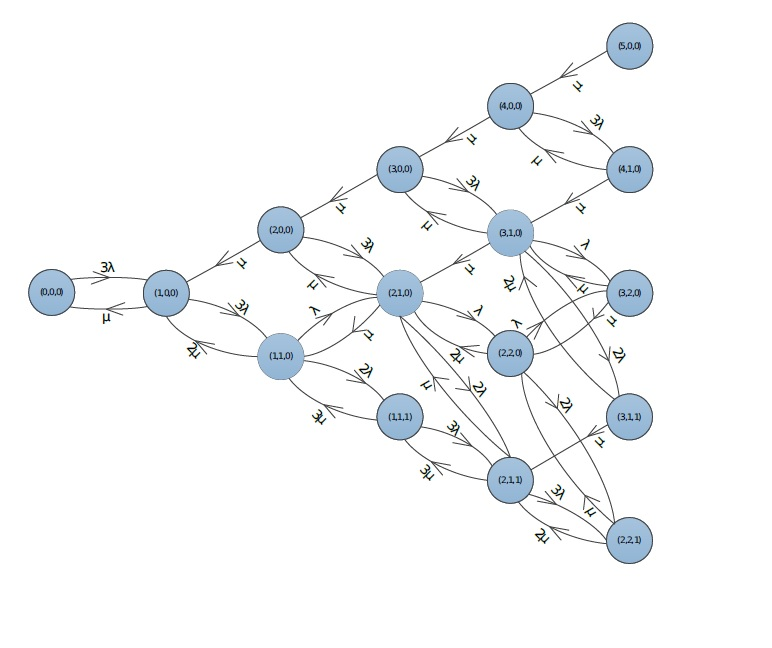
\includegraphics[scale=0.6]{Figures/1}
\caption{Original model.}
\label{fig:Orginal model.}
\end{figure}

\section{Lower and Upper bound Models:}
Now, we transform the original markov process by suitably redirecting the transitions such that the new generator matrices have some regular structure and whose analysis can be tackled by matrix analytic methods . The transformations are such that the average delays in the first and second transformed models are lower and upper bound respectively.
\\Both transformations have in common a threshold parameter and the following condition 
\begin{equation}
m_1-m_N\leq T \tag {3}
\end{equation}
\\As expected T adjusts accuracy of the models and higher T achieves tighter bounds at the expennse of numerical complexity.
\subsection{Lower Bound Model}
1. Arrivals which are violating (3) are sent to one of the shortest queues instead of longest.
2. When a departure causes violation of (3), departure occurs from the longest queue instead of the shortest queue.

\begin{figure}[h]
\centering
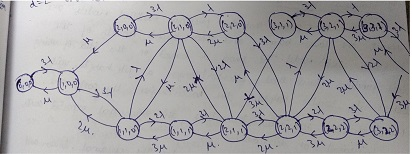
\includegraphics[scale=1]{Figures/lbm}
\caption{Lower bound model.}
\label{fig:Lower bound model.}

\end{figure}
\subsection{Upper Bound Model}
1.Whenever an arrival causes violation of eq(3), then the job arrival is accompanied by addition of one extra job at each of the shortest queues.
\\2.If a departure causes a violation, a depature may not occur.
\begin{figure}[h]
\centering
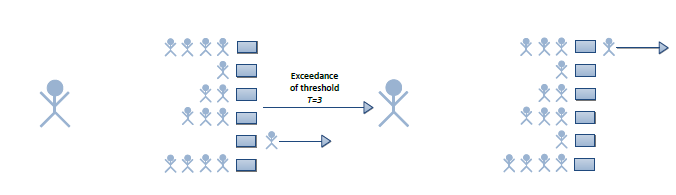
\includegraphics[scale=1]{Figures/ub}
\end{figure}
\subsection{Achieving Regularity}
The key advantage of the above transformations is to eliminate the irregularity in the original generator matrix Q and obtain new generator matrices with some regular structure. Now, we provide state diagrams of N=3 servers, d=2 choices and threshold T=2.
\begin{figure}[h]
\centering
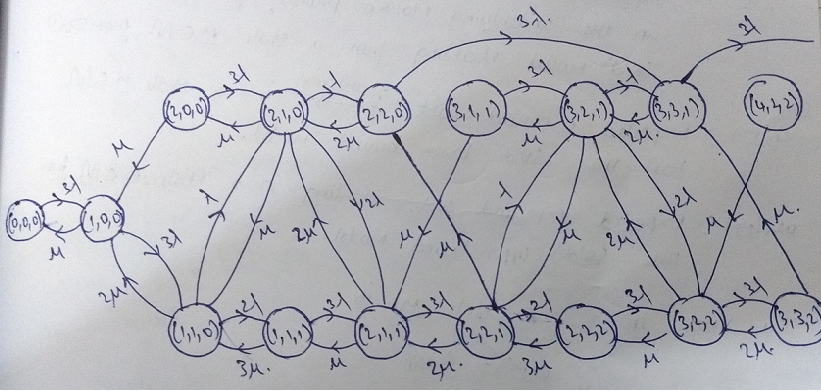
\includegraphics[scale=0.7]{Figures/ubm}
\caption{Upper bound model.}
\label{fig:Upper bound model.}
\end{figure}


Observe that, after some initial stages, the structure of the transition flow diagram repeats itselfi.e by observing set of states with 5, 6, 7 total number of jobs, the same structure of transition flow occurs even for set of states with 8, 9, 10 jobs.
\\The regularity of the transformed lower and upper bound models allows us to calculate a lower bound and upper bound of average delay by relying on matrix analytic methods. 

\section{Statistical Ordering}
Now we prove that the previous modified models are infact the lower bound and upper bound models of the original SQ(d) model. The proof is based on the idea of using cost functions such that shorter or longer a job has to wait before its service completion the lower or higher the costs are.
Moreover, the redirected transitions are such that expected costs are increased or decreased.
\\We now define the cost function for the original, lower and upper bound models.
\\$v_n(m)$ is the expected n-period cost at the embedded transition points in the underlying Markov process for the original SQ(d) model starting from a state m $\in$ M from equation (1).
\\$u_n(m)$ is the expected n-period cost starting in a state m $\in \mathcal{M}$ for the SQ(d) lower bound model.
\\$w_n(m)$ is the expected n- period cost starting in a state m $\in$ M for the SQ(d) upper bound model.
\\The cost in a given state M is 
\begin{align*}
C(M)=\sum_{i=1}^{N}m_i
\end{align*}
\\i.e., the total number of jobs in the system.
\\We assume that for all states M,$ u_0(M)=v_0(M)=w_0(M)=0$
\\The key to the proof is to show that for all states M and for all periods n
\begin{align*}
u_n(M)\le v_n(M)\le w_n(M) \tag{4}
\end{align*}                             
\subsection{For the upper bound model:}
We will proceed by induction on n. The case n=0 holds by definition with equality. Assuming equation (4) holds for some ($n\ge0$) we will prove it will also hold for n+1.
\\First we define simplifying ordering result on precedence pairs of states from $\mathcal{M}$ ordered in a suitable manner. Let M= $(m_1,….,m_N)$ and M'=$(m'_1,...,m'_N)$ for some states from  $\mathcal{M}$. We define precedence pairs
\begin{align*}
P = \{(M,M'): \sum_{i=1}^{j}m_i \le \sum_{i=1}^{N}m'_i  \text{       }\forall j=1,...N \}\\
\end{align*}
So, preferably the above inequalities can be interpreted as it is more favourable to have less number of jobs in the longest queues. On the other hand systems with fewer jobs have less expected cost and more balanced the system is, more efficient it will be and delays will be less.\\
Define $P_M$ as subset of P such that (M,M') with M' equal to $M+e_N1, M+e_1-e_2, M+e_2-e_3,......M+e_{N-1}-e_{N}$.\\
For some precedence pair (M,M') we define \\
\begin{align*}
d_i &= m'_i - m_i \text{     }\forall  1 \le i \le N.\\
S_j &=  \sum_{i=1}^{j}d_i  \text{       }\forall  j=1,...N.\\
\end{align*}
Then, one can write
\begin{align*}
 M = M'+S_Ne_N+S_{N-1}(e_{N-1}-e_{N})+.......+S1(e_1-e_2)\\
\end{align*}
where $e_i$ has all elements set to 0 except the $i^{th}$ element.\\
For any precedence pair (M,M') the M' has more number of jobs than M and infact in the longerqueues. Hence,

\begin{align*}
v_n(M) \le v_n(M') \text{    } \forall n \ge 0.\\
\end{align*}
The upper bound model is defined such that transitions are redirected to less attractive states i.e a transition to M' is directed to $\tilde{M'}$ such that $v_n(M) \le v_n(M')$.

Therefore we have,
\begin{align*}
v_{n+1}&=C(M)+\sum_{M'} p(M,M')v_n(M')\\
%\end{align*}
&\le C(M)+\sum_{\tilde M'}p(M,\tilde M')v_n(\tilde M')\\
&= C(M)+\sum_{\tilde M'}p(M,\tilde M')w_n(\tilde M')\\
&=w_{n+1}(M)\\
\end{align*}
By induction hypothesis, at every state the total number of jobs in the upper bound model will be greater than the lower bound model.
\subsection{For the lower bound model: }
As in the upper bound model model case, let us also define a procedence pair of states from $\mathcal{M}$ ordered in a suitable manner. For M=$(m_1,......m_N)$ and M'=$(m'_1,....m'_N)$ 
\begin{align*}
P = \{(M,M'): \sum_{i=1}^{j}m_i \ge \sum_{i=1}^{N}m'_i  \text{       }\forall j=1,...N \}\\
\end{align*}
i.e. the set P' may be interpreted as the pair of states M,M' where M has more number of customers than M' in its longest queues.
Hence M' has less cost and is infact more balanced than M. \\
Similar result $v_n(M) \ge v_n(M')$ as stated in the upper bound model exists ,So M' can be interpreted as the most favourable state than Min termms of cost function,\\
Therefore,$v_{n+1}=C(M)+\sum_{M'} p(M,M')v_n(M')$\\
Let $P'_M$ be a subset of P' such that M'=$M-e_N,M-e_1+e_2,... M-e_{N-1}+e_N$\\
Then for $\tilde{M'}$ from $P'_M$\\
\begin{align*}
v_{n+1}&=C(M)+\sum_{M'} p(M,M')v_n(M')\\
&\ge C(M)+\sum_{\tilde M'}p(M,\tilde M')v_n(\tilde M')\\
&= C(M)+\sum_{\tilde M'}p(M,\tilde M')w_n(\tilde M')\\
&=w_{n+1}(M)\\
\end{align*}
\section{Computation of equilibrium distribution and developing conditions for service time distribution insensitivity:}
Let 
\begin{align*}
P_k=\sum_{j \ge k} \pi_j\\
\end{align*}
i.e $P_k$ is equal to the asymptotic fraction of queues having atleast k jobs.\\
Since queue 1 with a state dependent poisson arrival process is a simple birth process, the flow balances equations give.\\
\begin{align*}
\pi_{k+1}&=\lambda_k \pi_k\\
\Rightarrow P_{k+1}-P_{k+2}&=\lambda_k (P_k-P_{k+1})\\
\lambda_k &=\lambda \frac{((P_k)^d-(P_{k+1})^d)}{(P_k-P_{k+1})}\\
\end{align*} 
 The above equation is for an SQ(d) policy with poisson arrival rate n$\lambda$\\
 Solving the above equations we get,\\
\begin{align*}
P_k= \lambda^{\frac{d^k-1}{d-1}}
\end{align*}
\subsection{General Service time insensitivity:}
The insensitivity of a policy refers to its indifference to the distribution of job service times and performance measures such as queue size distribution depend on service time distribution only through its mean.\\
It was found that, there exists a unique insensitive routing process characterized by $x=(x_1,x_2......x_n)$\\
Link i can serve a maximum of $N_i$ floors\\
$x_i$ is the number of floors on link i\\
$v_i{(x)} $is the actual arrival rate of link i,when network is in state x.\\
The routing algorithm will be insensitive if and only if ,\\
\begin{align*}
v_i{(x)}=\frac{N_i(x)-x_i}{\sum_{j=1}^{n}(N_j-x_j)}.\lambda\\ 
\end{align*}
Therefore,this is a greedy algorithm which routes floors at a rate proportional to capacity available at the queues.\\
This is not insensitive to service time probability distributions for any finite n.\\
But as n $\longrightarrow \infty$ an assuming the backlogs in each link become independent,\\
\begin{align*}
P_k&=\frac{\lambda^{\frac{d^{k}-1}{d-1}}}{\sum_{i=0}^{N}\lambda^\frac{d^{i}-1}{d-1}}\text{                    for k$\le N,$}\\
 P_k &=0\text{ for} k>N
\end{align*}

where N is capacity of each link.\\
Under all these assumptions the backlogs are insensitive to service time distribution.
The insensitivity also holds for sscheduing policies for premptive LIFO and other symmetric service disciplines.
\section{RESULT}
Little's law stats that 
\begin{align*}
\mathbb{E}[N] = \mathbb{E}[\lambda].\mathbb{E}[W]\\
\end{align*}

where N is the number of jobs in the system, $\lambda$ is the arrival rate and W is the waiting time of a job in the system.\\
Thus, as the number of customers increases the average delay also increases.\\
Our upper and lower bound models are designed such that 
$u_n(M) \le v_n(M) \le w_n(M)$\\
These lower and upper  bounds can be used to obtain lower and upper bound of delay performance.\\
Furthur using matrix analysis methods there is a scope to express the stationary distributions of upper and lower bounds in implicit form.\\


\section{Bibliography}

[1] Michael David Mitzenmacher. The Power of Two Choices in Randomized Load Balancing.B.A. (Harvard University).1991.\\

[2] I. J. B. F. Adan, J. Wessels, and W. H. M. Zijm. Analysis of the symmetric shortest queue problem. Stochastic Models, 6:691,713, 1990.\\

[3] I. J. B. F. Adan. A compensation approach for queueing problems. CWI (Centrum voor Wiskundeen Informatica),1994.\\

[4] M. Adler, S. Chakrabarti, M. Mitzenmacher, and L. Rasmussen. Parallel randomized load balancing. In Proceedings of the 27th ACM Symposium on the Theory of Computing, 1995.\\

[5] S.M. Ross. Stochastic Models. John Wiley and Sons, 1983\\



\end{document}